\section[Adv]{Advanced \cpp}

\subsection[OO]{Advanced OO}

\begin{frame}[fragile]
  \frametitlegb{Polymorphism}
  \begin{block}{the concept}
    \begin{itemize}
    \item objects actually have multiple types concurrently
    \item and can be used as any of them
    \end{itemize}
  \end{block}
  \begin{multicols}{2}
    \begin{cppcode*}{gobble=2}
      Polygon p;

      int f(Drawable & d) {...};
      f(p);  //ok

      try {
        throw p;
      } catch (Shape & e) {
        // will be caught
      }
    \end{cppcode*}
    \columnbreak
    \center
    \begin{tikzpicture}[node distance=1.5cm]
      \classbox{Drawable}{}
      \classbox[below of=Drawable]{Shape}{}
      \classbox[below of=Shape]{Polygon}{}
      \draw[very thick,->] (Polygon) -- (Shape);
      \draw[very thick,->] (Shape) -- (Drawable);
    \end{tikzpicture}
  \end{multicols}
\end{frame}


\begin{frame}[fragile]
  \frametitlegb{Inheritance privacy and polymorphism}
  \begin{block}{Only public inheritance is visible to code outside the class}
    \begin{itemize}
    \item private and protected are not
    \item this may restrict usage of polymorphism
    \end{itemize}
  \end{block}
  \begin{multicols}{2}
    \begin{cppcode*}{gobble=2}
      Polygon p;

      int f(Drawable & d) {...};
      f(p);  // Not ok anymore

      try {
        throw p;
      } catch (Shape & e) {
        // ok, will be caught
      }
    \end{cppcode*}
    \columnbreak
    \center
    \begin{tikzpicture}[node distance=1.5cm]
      \classbox{Drawable}{}
      \classbox[below of=Drawable]{Shape}{}
      \classbox[below of=Shape]{Polygon}{}
      \draw[very thick,->] (Polygon) -- (Shape) node[midway,right] {public};
      \draw[very thick,->] (Shape) -- (Drawable) node[midway,right] {private};
    \end{tikzpicture}
  \end{multicols}
\end{frame}

\begin{frame}[fragile]
  \frametitlegb{Method overriding}
  \begin{block}{the problem}
    \begin{itemize}
    \item a given method of the parent can be overriden in a child
    \item but which one is called ?
    \end{itemize}
  \end{block}
  \begin{multicols}{2}
    \begin{cppcode*}{gobble=2}
      Polygon p;
      p.draw(); // ?
      
      Shape & s = p;
      s.draw(); // ?
    \end{cppcode*}
    \columnbreak
    \center
    \begin{tikzpicture}[node distance=1.5cm]
      \classbox{Drawable}{
        void draw();
      }
      \classbox[below of=Drawable]{Shape}{}
      \classbox[below of=Shape]{Polygon}{
        void draw();
      }
      \draw[very thick,->] (Polygon) -- (Shape);
      \draw[very thick,->] (Shape) -- (Drawable);
    \end{tikzpicture}
  \end{multicols}
\end{frame}

\begin{frame}[fragile]
  \frametitlegb{Virtual methods}
  \begin{block}{the concept}
    \begin{itemize}
    \item methods can be declared {\it virtual}
    \item for these, the most precise object is always considered
    \item for others, the type of the variable decides
    \end{itemize}
  \end{block}
  \pause
  \begin{multicols}{2}
    \begin{cppcode*}{gobble=2}
      Polygon p;
      p.draw(); // Polygon.draw
      
      Shape & s = p;
      s.draw(); // Drawable.draw
    \end{cppcode*}
    \columnbreak
    \center
    \begin{tikzpicture}[node distance=1.5cm]
      \classbox{Drawable}{
        void draw();
      }
      \classbox[below of=Drawable]{Shape}{}
      \classbox[below of=Shape]{Polygon}{
        void draw();
      }
      \draw[very thick,->] (Polygon) -- (Shape);
      \draw[very thick,->] (Shape) -- (Drawable);
    \end{tikzpicture}
  \end{multicols}    
\end{frame}

\begin{frame}[fragile]
  \frametitlegb{Virtual methods}
  \begin{block}{the concept}
    \begin{itemize}
    \item methods can be declared {\it virtual}
    \item for these, the most precise object is always considered
    \item for others, the type of the variable decides
    \end{itemize}
  \end{block}
  \begin{multicols}{2}
    \begin{cppcode*}{gobble=2}
      Polygon p;
      p.draw(); // Polygon.draw
      
      Shape & s = p;
      s.draw(); // Polygon.draw
    \end{cppcode*}
    \columnbreak
    \center
    \begin{tikzpicture}[node distance=1.5cm]
      \classbox{Drawable}{
        virtual void draw();
      }
      \classbox[below of=Drawable]{Shape}{}
      \classbox[below of=Shape]{Polygon}{
        void draw();
      }
      \draw[very thick,->] (Polygon) -- (Shape);
      \draw[very thick,->] (Shape) -- (Drawable);
    \end{tikzpicture}
  \end{multicols}    
\end{frame}

\begin{frame}[fragile]
  \frametitleii{{\texttt override} keyword}
  \begin{block}{Principle}
    \begin{itemize}
    \item when overriding a virtual method
    \item the \mintinline{cpp}|override| keyword needs to be used
    \end{itemize}
  \end{block}
  \begin{exampleblock}{Practically}
    \begin{cppcode}
      struct Base {
        virtual void some_func(float);
      };
      struct Derived : Base {
        void some_func(float) override;
      };
    \end{cppcode}
  \end{exampleblock}
\end{frame}

\begin{frame}[fragile]
  \frametitleii{Why was {\texttt override} keyword introduced ?}
  To detect the mistake in the following code :
  \begin{block}{Without {\texttt override} (\cpp98)}
    \begin{cppcode}
      struct Base {
        virtual void some_func(float);
      };
      struct Derived : Base {
        void some_func(double); // oups !
      };
    \end{cppcode}
  \end{block}
  \begin{itemize}
  \item with \mintinline{cpp}|override|, you would get a compiler error
  \item if you forget \mintinline{cpp}|override| when you should have it, you get a compiler warning
  \end{itemize}
\end{frame}

\begin{frame}[fragile]
  \frametitleii{{\texttt final} keyword}
  \begin{block}{Idea}
    \begin{itemize}
    \item make sure you cannot override further a given virtual method
    \item by declaring it final
    \end{itemize}
  \end{block}
  \begin{exampleblock}{Practically}
    \begin{cppcode}
      struct Base {
        virtual void some_func(float);
      };
      struct Intermediate : Base {
        void some_func(float) final;
      };
      struct Derived : Intermediate {
        void some_func(float) override; // error
      };
    \end{cppcode}
  \end{exampleblock}
\end{frame}

\begin{frame}[fragile]
  \frametitlegb{Pure Virtual methods}
  \begin{block}{Concept}
    \begin{itemize}
    \item methods that exist but are not implemented
      \item marked by an ``{\it = 0} '' in the declaration
    \item makes their class abstract
    \item an object can only be instantiated for a non abstract class
    \end{itemize}
  \end{block}
  \pause
  \begin{multicols}{2}
    \begin{cppcode*}{gobble=2}
      // Error : abstract class
      Shape s;

      // ok, draw has been implemented
      Polygon p;
      
      // Shape type still usable
      Shape & s = p;
      s.draw();
    \end{cppcode*}
    \columnbreak
    \center
    \begin{tikzpicture}[node distance=1.5cm]
      \classbox{Drawable}{
        virtual void draw() = 0;
      }
      \classbox[below of=Drawable]{Shape}{}
      \classbox[below of=Shape]{Polygon}{
        void draw() override;
      }
      \draw[very thick,->] (Polygon) -- (Shape);
      \draw[very thick,->] (Shape) -- (Drawable);
    \end{tikzpicture}
  \end{multicols}
\end{frame}

\begin{frame}[fragile]
  \frametitlegb{Pure Abtract Class aka Interface}
  \begin{block}{Definition of pure abstract class}
    \begin{itemize}
    \item a class that has
      \begin{itemize}
        \item no data member
        \item all its methods pure virtual
      \end{itemize}
    \item the equivalent of an Interface in Java
    \end{itemize}
  \end{block}
  \begin{multicols}{2}
    \begin{cppcode*}{gobble=2}
      struct Drawable {
        virtual void draw() = 0;
      }
    \end{cppcode*}
    \columnbreak
    \center
    \begin{tikzpicture}[node distance=1.5cm]
      \classbox{Drawable}{
        virtual void draw() = 0;
      }
    \end{tikzpicture}
  \end{multicols}
\end{frame}

\begin{frame}[fragile]
  \frametitlegb{Overriding overloaded methods}
  \begin{block}{Concept}
    \begin{itemize}
    \item overriding an overloaded method will hide the others
    \item unless you inherit them using {\it using}
    \end{itemize}
  \end{block}
  \begin{cppcode*}{gobble=0}
    struct BaseClass {
      int foo(std::string);
      int foo(int);
    }
    struct DerivedClass : BaseClass {
      using BaseClass::foo;
      int foo(std::string);
    }
    DerivedClass dc;
    dc.foo(4);      // error if no using
    \end{cppcode*}
\end{frame}

\begin{frame}[fragile]
  \frametitlegb{Polymorphism}
  \begin{alertblock}{Exercise Time}
    \begin{itemize}
    \item go to code/polymorphism
    \item look at the code
    \item open test.cpp
    \item create a Pentagon, call its perimeter method
    \item create an Hexagon, call its perimeter method
    \item create an Hexagon, call its parent's perimeter method
    \item retry with virtual methods
    \end{itemize}
  \end{alertblock}
\end{frame}

\begin{frame}[fragile]
  \frametitlegb{Multiple Inheritance}
  \begin{block}{Concept}
    \begin{itemize}
    \item one class can inherit from multiple parents
    \end{itemize}
  \end{block}
  \begin{multicols}{2}
    \begin{tikzpicture}[]
      \classbox[]{Polygon}{}
      \classbox[below of=Polygon,node distance=1.5cm]{Rectangle}{}
      \classbox[right of=Rectangle,node distance=3cm]{Text}{}
      \classbox[below right of=Rectangle,node distance=2cm]{TextBox}{}
      \draw[very thick,->] (Polygon) -- (Rectangle);
      \draw[very thick,->] (Rectangle) -- (TextBox);
      \draw[very thick,->] (Text) -- (TextBox);
    \end{tikzpicture}
    \columnbreak
    \vspace{2cm}
    \begin{cppcode*}{gobble=2}
      class TextBox :
        public Rectangle, Text {
        // inherits of both
      }
    \end{cppcode*}
  \end{multicols}
\end{frame}

\begin{frame}[fragile]
  \frametitlegb{The diamond shape}
  \begin{block}{Definition}
    \begin{itemize}
    \item situation when one class inherits several times from a given grand parent
    \end{itemize}
  \end{block}
  \begin{alertblock}{Problem}
    \begin{itemize}
    \item are the members of the grand parent replicated ?
    \end{itemize}
  \end{alertblock}
  \vfill
  \hspace{2.5cm}
  \begin{tikzpicture}[]
    \classbox[]{Drawable}{}
    \classbox[below left of=Drawable,node distance=2cm]{Rectangle}{}
    \classbox[right of=Rectangle,node distance=3cm]{Text}{}
    \classbox[below right of=Rectangle,node distance=2cm]{TextBox}{}
    \draw[very thick,->] (Drawable) -- (Rectangle);
    \draw[very thick,->] (Drawable) -- (Text);
    \draw[very thick,->] (Rectangle) -- (TextBox);
    \draw[very thick,->] (Text) -- (TextBox);
  \end{tikzpicture}
\end{frame}

\begin{frame}[fragile]
  \frametitlegb{Virtual inheritance}
  \begin{block}{Solution}
    \begin{itemize}
    \item inheritance can be {\it virtual} or not
    \item {\it virtual} inheritance will ``share'' parents
    \item standard inheritance will replicate them
    \end{itemize}
    \mintinline{cpp}{class TextBox : public virtual Rectangle, Text}
  \end{block}
  \begin{multicols}{2}
    \begin{tikzpicture}[]
      \draw node (title) [rectangle] {virtual};
      \classbox[below of=title]{Drawable}{}
      \classbox[below left of=Drawable,node distance=2cm]{Rectangle}{}
      \classbox[right of=Rectangle,node distance=3cm]{Text}{}
      \classbox[below right of=Rectangle,node distance=2cm]{TextBox}{}
      \draw[very thick,->] (Drawable) -- (Rectangle);
      \draw[very thick,->] (Drawable) -- (Text);
      \draw[very thick,->] (Rectangle) -- (TextBox);
      \draw[very thick,->] (Text) -- (TextBox);
    \end{tikzpicture}
    \columnbreak
    \begin{tikzpicture}[]
      \classbox[]{Drawable1}{}
      \classbox[below of=Drawable1,node distance=1.5cm]{Rectangle}{}
      \draw[very thick,->] (Drawable1) -- (Rectangle);
      \classbox[right of=Drawable1,node distance=3cm]{Drawable2}{}
      \classbox[below of=Drawable2,node distance=1.5cm]{Text}{}
      \draw[very thick,->] (Drawable2) -- (Text);
      \classbox[below right of=Rectangle,node distance=2cm]{TextBox}{}
      \draw[very thick,->] (Rectangle) -- (TextBox);
      \draw[very thick,->] (Text) -- (TextBox);
      \draw node at (1.5cm,1cm) [rectangle] {standard};
    \end{tikzpicture}
  \end{multicols}
\end{frame}

\begin{frame}[fragile]
  \frametitlegb{Multiple inheritance advice}
  \begin{block}{Do not use multiple inheritance}
    \begin{itemize}
    \item Except for inheriting from interfaces
    \item and for very seldom special cases
    \end{itemize}
  \end{block}
  \pause
  \begin{alertblock}{Do not use diamond shapes}
    \begin{itemize}
    \item This is a sign that your architecture is not correct
    \item In case you are tempted, think twice and change mind
    \end{itemize}
  \end{alertblock}
\end{frame}

\begin{frame}[fragile]
  \frametitlegb{Virtual inheritance}
  \begin{alertblock}{Exercise Time}
    \begin{itemize}
    \item go to code/virtual\_inheritance
    \item look at the code
    \item open test.cpp
    \item create a TextBox and call draw
    \item Fix the code to call both draws by using types
    \item retry with virtual inheritance
    \end{itemize}
  \end{alertblock}
\end{frame}

\begin{frame}[fragile]
  \frametitlegb{Virtual inheritance}
  \begin{alertblock}{Warning}
    in case of virtual inheritance it is the most derived class that calls the virtual base class' constructor
  \end{alertblock}
\end{frame}


\subsection{Operators}

\begin{frame}[fragile]
  \frametitlegb{Operators' example}
  \begin{cppcode}
    struct Complex {
      float m_real, m_imaginary;
      Complex(float real, float imaginary);
      Complex operator+(const Complex& other) {
        return Complex(m_real + other.m_real,
                       m_imaginary + other.m_imaginary);
      }
    }

    Complex c1(2, 3), c2 (4, 5);
    Complex c3 = c1 + c2; // (6, 8)
  \end{cppcode}
\end{frame}

\begin{frame}
  \frametitlegb{Operators}
  \begin{block}{Definition for operators of a class}
    \begin{itemize}
    \item implemented as a regular method
      \begin{itemize}
      \item either inside the class, as a member function
      \item or outside the class (not all)
      \end{itemize}
    \item with a special name (replace @ by anything)
      \begin{tabular}{llll}
        Expression & As member & As non-member \\
        \hline
        @a & (a).operator@() & operator@(a) \\
        a@b & (a).operator@(b) & operator@(a,b) \\
        a=b & (a).operator=(b) & cannot be non-member \\
        a(b...) & (a).operator()(b...) & cannot be non-member \\
        a[b] & (a).operator[](b) & cannot be non-member \\
        a-\textgreater & (a).operator-\textgreater() & cannot be non-member \\
        a@ & (a).operator@(0) & operator@(a,0) \\
      \end{tabular}
    \end{itemize}
  \end{block}
\end{frame}

\begin{frame}[fragile]
  \frametitlegb{Why to have non-member operators ?}
  \begin{block}{Symetry}
    \begin{cppcode}
      struct Complex {
        float m_real, m_imaginary;
        Complex operator+(float other) {
          return Complex(m_real + other, m_imaginary);
        }
      }
      Complex c1(2, 3);
      Complex c2 = c1 + 4;  // ok
      Complex c3 = 4 + c1;  // not ok !!
    \end{cppcode}
    \pause
    \begin{cppcode*}{firstnumber=10}
      Complex operator+(float a, const Complex& obj) {
        return Complex(a + obj.m_real, obj.m_imaginary);
      }
    \end{cppcode*}
  \end{block}
\end{frame}

\begin{frame}[fragile]
  \frametitlegb{Other reason to have non-member operators ?}
  \begin{block}{Extending existing classes}
    \begin{cppcode}
      struct Complex {
        float m_real, m_imaginary;
        Complex(float real, float imaginary);
      }

      std::ostream& operator<<(std::ostream& os,
                               const Complex& obj) {
        os << "(" << obj.m_real << ", "
                  << obj.m_imaginary << ")";
        return os;
      }
      Complex c1(2, 3);
      std::cout << c1 << std::endl;
    \end{cppcode}
  \end{block}
\end{frame}

\subsection[Functors]{Functors}

\begin{frame}[fragile]
  \frametitlegb{Functors}
  \begin{block}{Concept}
    \begin{itemize}
    \item a class that implements the () operator
    \item allows to use objects in place of functions
    \item and as objects have constructors, allow to construct functions
    \end{itemize}
  \end{block}
  \begin{cppcode}
    struct Adder {
      int m_increment;
      Adder(int increment) : m_increment(increment) {}
      int operator()(int a) { return a + m_increment; }
    };

    Adder inc1(1), inc10(10);
    int i = 3;
    int j = inc1(i);  // 4
    int k = inc10(i); // 13
  \end{cppcode}
\end{frame}

\begin{frame}[fragile]
  \frametitlegb{Functors}
  \begin{block}{Typical usage}
    \begin{itemize}
    \item pass a function to another one
    \item or to an STL algorithm
    \end{itemize}
  \end{block}
  \begin{cppcode}
    struct BinaryFunction {
      virtual double operator() (double a, double b) = 0;
    };
    struct Add : public BinaryFunction {
      double operator() (double a, double b) { return a+b; }
    };
    double binary_op(double a, double b, BinaryFunction &func) {
      return func(a, b);
    }
    Add addfunc;
    double c = binary_op(a, b, addfunc);
  \end{cppcode}
\end{frame}

\subsection[\textless{}T\textgreater]{Templates}

\begin{frame}[fragile]
  \frametitlegb{Templates}
  \begin{block}{Concept}
    \begin{itemize}
    \item The \cpp way to write reusable code
      \begin{itemize}
        \item aka macros on steroids
      \end{itemize}
    \item Applicable to functions and objects
    \end{itemize}
  \end{block}
  \begin{cppcode}
    template<class T>
    const T & Max(const T &A, const T &B) {
      return A > B ? A : B;
    }

    template<class T>
    struct Vector {
      int m_len;
      T* m_data;
    }
 \end{cppcode}
\end{frame}

\begin{frame}[fragile]
  \frametitlegb{Templates}
  \begin{alertblock}{Warning}
    These are really like macros
    \begin{itemize}
      \item they are compiled n times
      \item they need to be defined before used
      \begin{itemize}
        \item so all templated code has to be in headers
      \end{itemize}
      \item this may lead to longer compilation times and bigger libraries
    \end{itemize}
  \end{alertblock}
  \newsavebox{\codepiece}
  \begin{lrbox}{\codepiece}
    \begin{minipage}{.35\linewidth}
      \begin{cppcode*}{gobble=4}
        template<class T>
        T func(T a) {
          return a;
        }
      \end{cppcode*}
    \end{minipage}
  \end{lrbox}
  \newsavebox{\codepiecea}
  \begin{lrbox}{\codepiecea}
    \begin{minipage}{.4\linewidth}
      \begin{cppcode*}{gobble=4}
        int func(int a) {
          return a;
        }
      \end{cppcode*}
    \end{minipage}
  \end{lrbox}
  \newsavebox{\codepieceb}
  \begin{lrbox}{\codepieceb}
    \begin{minipage}{.4\linewidth}
      \begin{cppcode*}{gobble=4}
        double func(double a) {
          return a;
        }
      \end{cppcode*}
    \end{minipage}
  \end{lrbox}
  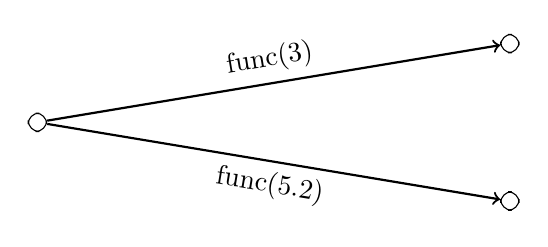
\begin{tikzpicture}[rectangle,rounded corners]
    \draw node (template) [draw] {\usebox{\codepiece}}
          node (templatea) [draw] at (6cm,+1cm) {\usebox{\codepiecea}}
          node (templateb) [draw] at (6cm,-1cm) {\usebox{\codepieceb}};
    \draw[->,thick] (template) -- (templatea) node [above,midway,sloped] {func(3)};
    \draw[->,thick] (template) -- (templateb) node [below,midway,sloped] {func(5.2)};
  \end{tikzpicture}
\end{frame}

\begin{frame}[fragile]
  \frametitlegb{Templates}
  \begin{block}{Arguments}
    \begin{itemize}
    \item can be a class, 
    \item you can have several
    \item last ones can have a default value
    \end{itemize}
  \end{block}
  \begin{cppcode*}{}
    template<class KeyType=int, class ValueType=KeyType>
    struct Map {
      void set(const KeyType &key, ValueType value);
      ValueType get(const KeyType &key);
    }

    Map<std::string, int> m1;
    Map<float> m2;   // Map<float, float>
    Map<> m3;        // Map<int, int>
  \end{cppcode*}
\end{frame}

\begin{frame}[fragile]
  \frametitlegb{Templates implementation}
  \begin{cppcode*}{}
    template<class KeyType=int, class ValueType=KeyType>
    struct Map {
      void set(const KeyType &key, ValueType value);
      ValueType get(const KeyType &key);
    }

    template<class KeyType, class ValueType>
    void Map<KeyType, ValueType>::set
       (const KeyType &key, ValueType value) {
      ...
    }

    template<class KeyType, class ValueType>
    ValueType Map<KeyType, ValueType>::get
       (const KeyType &key) {
      ...
    }
  \end{cppcode*}
\end{frame}

\begin{frame}[fragile]
  \frametitlegb{Templates}
  \begin{block}{Specialization}
    templates can be specialized for given values of their parameter
  \end{block}
  \begin{cppcode*}{}
    template<unsigned int N> struct Polygon {
      Polygon(float radius);
      float perimeter();
      float m_radius;
    };
    
    template<>
    struct Polygon<6> {
      Polygon(float radius);
      float perimeter() {return 6*m_radius;};
      float m_radius;
    };
  \end{cppcode*}
\end{frame}

\begin{frame}[fragile]
  \frametitlegb{The full power of templates}
  \begin{alertblock}{Exercise Time}
    \begin{itemize}
    \item go to code/template
    \item look at the OrderedVector code
    \item compile and run test.cpp. See the ordering
    \item modify test.cpp and reuse OrderedVector with Complex
    \item improve OrderedVector to template the ordering
    \item test reverse ordering of strings (from the last letter)
    \item test manhattan order with complex type
    \item check the implementation of Complex
    \item try ordering complex of complex
    \end{itemize}
  \end{alertblock}
\end{frame}

\subsection[STL]{The STL}

\begin{frame}[fragile]
  \frametitlegb{The Standard Template Library}
  \begin{block}{What it is}
    \begin{itemize}
    \item A library of standard templates
    \item Everything you need, or ever dreamed of
      \begin{itemize}
      \item strings, containers, iterators
      \item algorithms, functions, sorters
      \item functors, allocators
      \item ...
      \end{itemize}
    \item Portable
    \item Reusable
    \item Efficient
    \end{itemize}
  \end{block}
  \pause
  \begin{alertblock}{Just use it}
    and adapt it to your needs, thanks to templates
  \end{alertblock}
\end{frame}

\begin{frame}[fragile,label=STLcode]
  \frametitleii{STL in practice}
  \begin{cppcode*}{}
    #include <vector>
    #include <algorithm>

    std::vector<int> vi{5, 3, 4}; // initializer list
    std::vector<int> vr(3); // constructor taking int

    std::transform(vi.begin(), vi.end(),      // range1
                   vi.begin(),          // start range2
                   vr.begin(),          // start result
                   std::multiplies<int>()); // function

    for(auto n : vr) {
      std::cout << n << " ";
    };
  \end{cppcode*}
\end{frame}

\begin{frame}[fragile]
  \frametitlegb{STL's concepts}
  \begin{block}{containers}
    \begin{itemize}
    \item a structure containing data
    \item with a given way of handling it
    \item irrespective of
      \begin{itemize}
      \item the data itself (templated)
      \item the memory allocation of the structure (templated)
      \item the algorithms that may use the structure
      \end{itemize}
    \item examples
      \begin{itemize}
      \item string
      \item tuple, list, vector, deque
      \item map, set, multimap, multiset, hash\_map, hash-set, ...
      \item stack, queue, priority\_queue
      \end{itemize}
    \end{itemize}
  \end{block}
\end{frame}

\begin{frame}[fragile]
  \frametitlegb{STL's concepts}
  \begin{block}{iterators}
    \begin{itemize}
    \item generalization of pointers
    \item allowing iteration over some data
    \item irrespective of
      \begin{itemize}
      \item the container used (templated)
      \item the data itself (container is templated)
      \item the consumer of the data (templated algorithm)
      \end{itemize}
    \item examples
      \begin{itemize}
      \item iterator
      \item reverse\_iterator
      \item const\_iterator
      \end{itemize}
    \end{itemize}
  \end{block}
\end{frame}

\begin{frame}[fragile]
  \frametitlegb{STL's concepts}
  \begin{block}{algorithms}
    \begin{itemize}
    \item implementation of an algorithm working on data
    \item with a well defined behavior (defined complexity)
    \item irrespective of
      \begin{itemize}
      \item the data handled
      \item the container where data live
      \item the iterator used to go through data
      \end{itemize}
    \item examples
      \begin{itemize}
      \item for\_each, find, find\_if, count, count\_if, search
      \item copy, swap, transform, replace, fill, generate
      \item remove, remove\_if
      \item unique, reverse, rotate, random, partition
      \item sort, partial\_sort, merge, min, max
      \item lexicographical\_compare, iota, accumulate, partial\_sum
      \end{itemize}
    \end{itemize}
  \end{block}
\end{frame}
      
\begin{frame}[fragile]
  \frametitlegb{STL's concepts}
  \begin{block}{functions / functors}
    \begin{itemize}
      \item generic utility functions/functors
      \item mostly useful to be passed to STL algorithms
    \item implemented independently of
      \begin{itemize}
      \item the data handled (templated)
      \item the context (algorithm) calling it
      \end{itemize}
    \item examples
      \begin{itemize}
      \item plus, minus, multiply, divide, modulus, negate
      \item equal\_to, less, greater, less\_equal, ...
      \item logical\_and, logical\_or, logical\_not
      \item identity, project1st, project2nd
      \item binder1st, binder2nd, unary\_compose, binary\_compose
      \end{itemize}
    \end{itemize}
  \end{block}
\end{frame}

\againframe{STLcode}

\begin{frame}[fragile]
  \frametitlegb{STL in practice using \cpp98}
  \begin{cppcode*}{}
    #include <vector>
    #include <algorithm>

    std::vector<int> vi, vr(3);
    vi.push_back(5); vi.push_back(3); vi.push_back(4);

    std::transform(vi.begin(), vi.end(),      // range1
                   vi.begin(),          // start range2
                   vr.begin(),          // start result
                   std::multiplies<int>()); // function

    for(std::vector<int>::iterator it = vr.begin();
        it != vr.end();
        it++) {
      std::cout << *it << " ";
    };
  \end{cppcode*}
\end{frame}

\begin{frame}[fragile]
  \frametitlegb{STL and functors}
  \begin{cppcode}
    // Finds the first element in a list that lies in
    // the range from 1 to 10.
    list<int> L;
    ...
    list<int>::iterator in_range = 
      find_if(L.begin(), L.end(),
              compose2(logical_and<bool>(),
                       bind2nd(greater_equal<int>(), 1),
                       bind2nd(less_equal<int>(), 10)));

    // Computes sin(x)/(x + DBL_MIN) for elements of a range.
    transform(first, last, first,
              compose2(divides<double>(),
                       ptr_fun(sin),
                       bind2nd(plus<double>(), DBL_MIN)));
  \end{cppcode}
\end{frame}

\begin{frame}[fragile]
  \frametitlegb{Welcome to lego programming !}
  \begin{block}{}
    \pgfdeclareimage[height=0.5cm]{AtlasLego}{AtlasLego.jpg}
    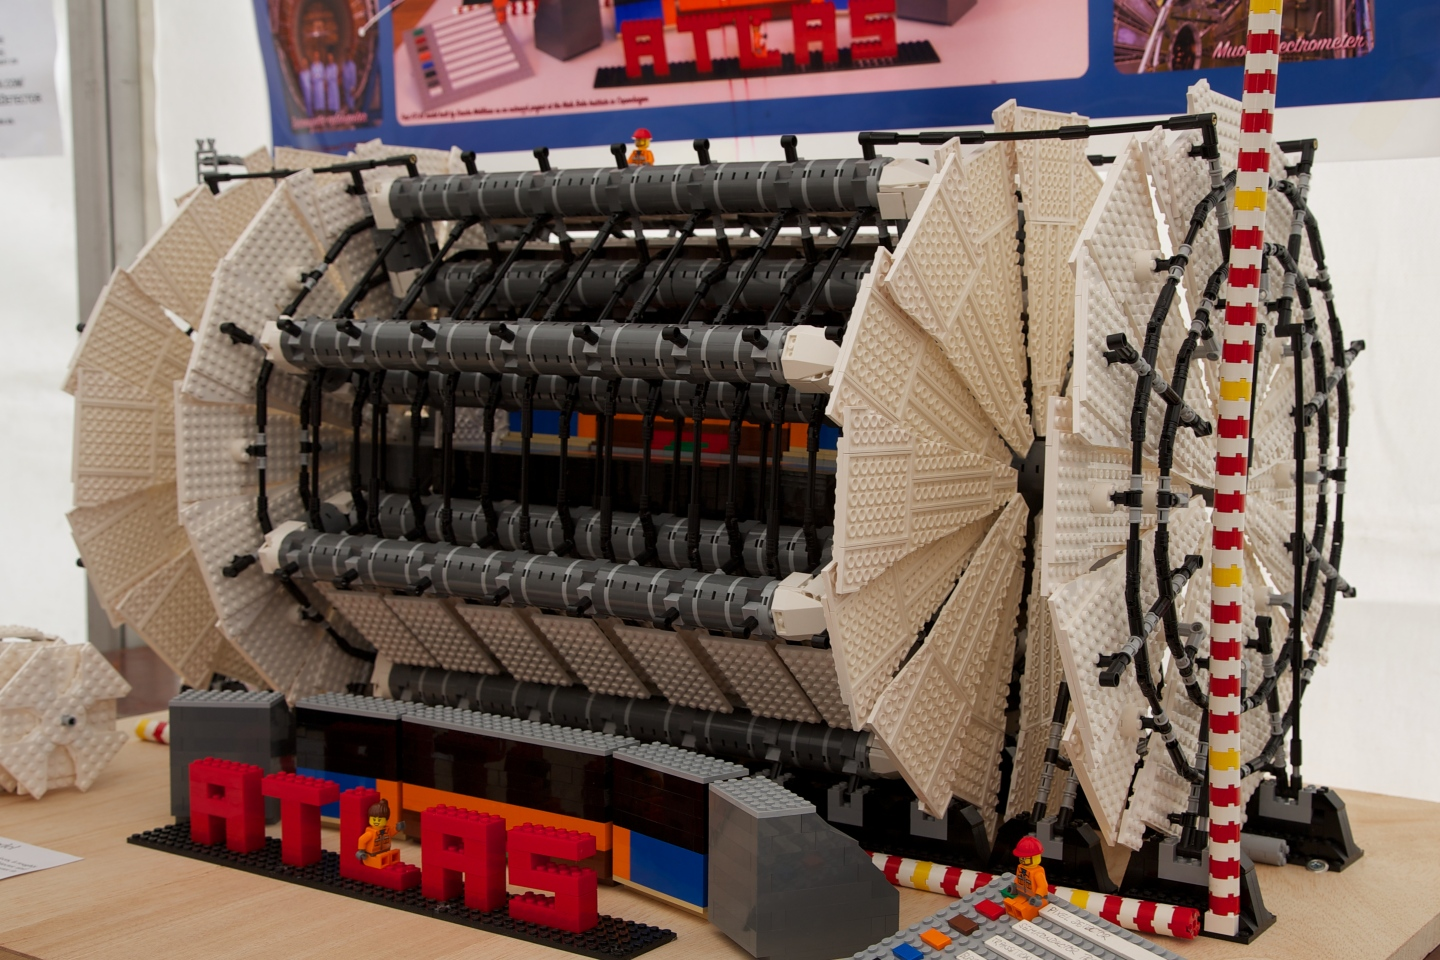
\includegraphics[width=\linewidth]{AtlasLego}
  \end{block}
\end{frame}

\begin{frame}[fragile]
  \frametitlegb{Using the STL}
  \begin{alertblock}{Exercise Time}
    \begin{itemize}
    \item go to code/stl
    \item look at the non STL code in test.nostl.cpp 
      \begin{itemize}
        \item it creates a vector of ints at regular intervals
        \item it randomizes them
        \item it computes differences between consecutive ints
        \item and the mean and variance of it
      \end{itemize}
    \item open test.cpp and complete the ``translation'' to STL
    \item see how easy it is to reuse the code with complex numbers
    \end{itemize}
  \end{alertblock}
\end{frame}

\begin{frame}[fragile]
  \frametitlegb{Using the STL}
  \begin{alertblock}{Some last warning}
    You may find the STL quite difficult to use.
    \begin{itemize}
    \item template syntax is simply awful
    \item it is hard to debug (compilers spit out mostly garbage)
    \end{itemize}
    However, this has improved a lot with \cpp11
  \end{alertblock}
\end{frame}

\begin{frame}[fragile]
  \frametitleii{Loops and auto keyword with the STL}
  \begin{block}{Old way}
    \begin{cppcode*}{}
      std::vector<int> a = ...;
      int sum = 0;
      for (std::vector<int>::iterator it = v.begin();
           it != v.end(); it++) {
        sum += *it;
      }
    \end{cppcode*}
  \end{block}
  \pause
  \begin{block}{New way}
    \begin{cppcode*}{}
      std::vector<int> v = ...;
      int sum = 0;
      for (auto a : v) { sum += a; }
    \end{cppcode*}
  \end{block}
  \pause
  \begin{exampleblock}{STL way}
    \begin{cppcode*}{}
      std::vector<int> v = ...;
      int sum = std::accumulate(v.begin(), v.end(), 0);
    \end{cppcode*}
  \end{exampleblock}
\end{frame}

\subsection{More STL}

\begin{frame}[fragile]
  \frametitleit{Some new STL types}
  \begin{block}{\texttt{std::optional}}
    \begin{itemize}
    \item manages an optional contained value
    \item contextually converted to bool
    \item useful for the return value of a function that may fail
    \end{itemize}
  \end{block}
  \begin{block}{\texttt{std::any}}
    \begin{itemize}
    \item a type-safe container for single values of any type
    \item the \texttt{any\_cast} function provides type-safe access
    \item and throws \texttt{std::bad\_any\_cast} for bad access
    \end{itemize}
  \end{block}
  \begin{block}{\texttt{std::variant}}
    \begin{itemize}
    \item a type-safe union
    \item \texttt{std::get} reads the value of the variant
    \item and throws \texttt{std::bad\_variant\_access} for bad accesses
    \end{itemize}
  \end{block}
\end{frame}

\begin{frame}[fragile]
  \frametitleii{non-member begin and end}
  \begin{alertblock}{The problem in \cpp98}
    STL containers and arrays have different syntax for loop
    \vspace{-1mm}
    \begin{cppcode}
      std::vector<int> v;
      int a[] = {1,2,3};
      for(auto it = v.begin(); it != v.end(); it++) {...}
      for(int i = 0; i < 3; i++) {...}
    \end{cppcode}
  \end{alertblock}
  \pause
  \begin{block}{A new syntax}
    \begin{cppcode}
      for(auto it = begin(v); it != end(v); it++) {...}
      for(auto i = begin(a); i != end(a); i++) {...}
    \end{cppcode}
  \end{block}
  \pause
  \begin{exampleblock}{Allowing the best syntax}
    \begin{cppcode}
      for(auto & element : v) {...}
      for(auto & element : a) {...}
    \end{cppcode}
  \end{exampleblock}
\end{frame}

\begin{frame}[fragile]
  \frametitleit{Structured Binding Declarations}
  Helps when using tuples as a return type.\\
  Automatically creates variables and ties them.
  \begin{alertblock}{\cpp14}
    \begin{cppcode*}{}
      void foo(std::tuple<int, double, long> tuple) {
        int a = 0;
        double b = 0.0;
        long c = 0;
        // a, b, c need to be declared first
        std::tie(a, b, c) = tuple;
    \end{cppcode*}
  \end{alertblock}
  \begin{exampleblock}{\cpp17}
    \begin{cppcode*}{}
      void foo(std::tuple<int, double, long> tuple) {
      auto [ a, b, c ] = tuple;
    \end{cppcode*}
  \end{exampleblock}
\end{frame}

\subsection[$\lambda$]{Lambdas}

\begin{frame}[fragile]
  \frametitleii{Function return type}
  \begin{block}{A new way to specify function's return type}
    \begin{cppcode*}{linenos=false}
      ReturnType fn_name(ArgType1, ArgType2);  //old
      auto fn_name(ArgType1, ArgType2) -> ReturnType;
    \end{cppcode*}
  \end{block}
  \pause
  \begin{block}{Advantages}
    \begin{itemize}
    \item Allows to simplify inner type definition
      \begin{cppcode*}{gobble=4}
        class TheClass {
          using inner_type = int;
          inner_type func();
        }
        TheClass::inner_type TheClass::func() {...}
        auto TheClass::func() -> inner_type {...}
      \end{cppcode*}
    \item will be used for lambdas
    \end{itemize}
  \end{block}
\end{frame}


\begin{frame}[fragile]
  \frametitleii{Lambdas}
  \begin{block}{Definition}
    a lambda is a function with no name
  \end{block}
  \pause
  \begin{exampleblock}{Python example}
    \begin{pythoncode*}{}
      data = [1,9,3,8,3,7,4,6,5]

      # without lambdas
      def isOdd(n):
        return n%2 == 1
      print filter(isOdd, data)

      # with lambdas
      print filter(lambda n:n%2==1, data)
    \end{pythoncode*}
  \end{exampleblock}
\end{frame}

\begin{frame}[fragile]
  \frametitleii{\cpp Lambdas}
  \begin{block}{Simplified syntax}
    \begin{cppcode*}{gobble=2}
      [] (args) -> type {
        code;
      }
    \end{cppcode*}
    The type specification is optional
  \end{block}
  \begin{exampleblock}{Usage example}
    \begin{cppcode*}{gobble=2}
      std::vector<int> data{1,2,3,4,5};
      for_each(begin(data), end(data),
               [](int i) {
                 std::cout << "The square of " << i
                           << " is " << i*i << std::endl;
               });
    \end{cppcode*}
  \end{exampleblock}
\end{frame}


\begin{frame}[fragile]
  \frametitleii{Capture}
  \begin{block}{Python code}
    \begin{pythoncode*}{}
      increment = 3
      data = [1,9,3,8,3,7,4,6,5]
      map(lambda x : x + increment, data)
    \end{pythoncode*}
  \end{block}
  \pause
  \begin{block}{First attempt in \cpp}
    \begin{cppcode}
      int increment = 3;
      std::vector<int> data{1,9,3,8,3,7,4,6,5};
      transform(begin(data), end(data), begin(data),
                [](int x) { return x+increment; });
    \end{cppcode}
  \end{block}
  \pause
  \begin{alertblock}{Error}
    \begin{minted}[gobble=6]{text}
        error: 'increment' is not captured
          [](int x) { return x+increment; });
                                     ^
    \end{minted}
  \end{alertblock}
\end{frame}

\begin{frame}[fragile]
  \frametitleii{Capture}
  \begin{block}{Variable capture}
    \begin{itemize}
    \item external variables need to be explicitely captured
    \item captured variables are listed within initial []
    \end{itemize}
  \end{block}
  \pause
  \begin{exampleblock}{Example}
    \begin{cppcode*}{}
      int increment = 3;
      std::vector<int> data{1,9,3,8,3,7,4,6,5};
      transform(begin(data), end(data), begin(data),
                [increment](int x) {
                  std::cout << x+increment;
                });
    \end{cppcode*}
  \end{exampleblock}
\end{frame}

\begin{frame}[fragile]
  \frametitleii{Default capture is by value}
  \begin{exampleblock}{Code example}
    \begin{cppcode}
      int sum = 0;
      std::vector<int> data{1,9,3,8,3,7,4,6,5};
      for_each(begin(data), end(data),
              [sum](int x) { sum += x; });
    \end{cppcode}
  \end{exampleblock}
  \pause
  \begin{alertblock}{Error}
    \begin{minted}[gobble=4]{text}
      error: assignment of read-only variable 'sum'
               [sum](int x) { sum += x; });
    \end{minted}
  \end{alertblock}
  \pause
  \begin{block}{Explanation}
    By default, variables are captured by value
  \end{block}
\end{frame}

\begin{frame}[fragile]
  \frametitleii{Capture by reference}
  \begin{exampleblock}{Simple example}
    In order to capture by reference, add '\&' before the variable
    \begin{cppcode}
      int sum = 0;
      std::vector<int> data{1,9,3,8,3,7,4,6,5};
      for_each(begin(data), end(data),
              [&sum](int x) { sum += x; });
    \end{cppcode}
  \end{exampleblock}
  \pause
  \begin{exampleblock}{Mixed case}
    One can of course mix values and references
    \begin{cppcode}
      int sum = 0, offset = 1;
      std::vector<int> data{1,9,3,8,3,7,4,6,5};
      for_each(begin(data), end(data),
              [&sum, offset](int x) {
                sum += x + offset;
              });
    \end{cppcode}
  \end{exampleblock}
\end{frame}

\begin{frame}[fragile]
  \frametitleii{Capture all}
  \begin{block}{by value}
    \begin{cppcode*}{linenos=false}
      [=](...) { ... };
    \end{cppcode*}
  \end{block}
  \pause
  \begin{block}{by reference}
    \begin{cppcode*}{linenos=false}
      [&](...) { ... };
    \end{cppcode*}
  \end{block}
  \pause
  \begin{block}{exceptions}
    \begin{cppcode*}{linenos=false}
      [&, b](...) { ... };
      [=, &b](...) { ... };
    \end{cppcode*}
  \end{block}
\end{frame}

\begin{frame}[fragile]
  \frametitleii{Closures}
  \begin{exampleblock}{Example}
    \begin{cppcode*}{}
      auto build_incrementer = [](int inc) {
        return [inc](int value) { return value + inc; };
      };
      auto inc1 = build_incrementer(1);
      auto inc10 = build_incrementer(10);
      int i = 0;
      i = inc1(i);   // i = 1
      i = inc10(i);  // i = 11
    \end{cppcode*}
  \end{exampleblock}
  \begin{block}{How it works}
    \begin{itemize}
      \item build\_incrementer returns a function object
      \item this function's behavior depends on a parameter
      \item note how {\it auto} is useful here !
    \end{itemize}
  \end{block}
\end{frame}

\begin{frame}[fragile]
  \frametitleii{{\texttt lambda}s makes the STL usable}
  \begin{block}{Before lambdas}
    \begin{cppcode*}{}
      struct Incrementer {
        int m_inc;
        Incrementer(int inc) : m_inc(inc) {}
        int operator() (int value) {
          return value + m_inc;
        };
      };
      std::vector<int> v{1, 2, 3};
      std::transform(begin(v), end(v), begin(v),
                     Incrementer(1));
      for (auto a : v) std::cout << a << " ";
      \end{cppcode*}
    \end{block}
\end{frame}

\begin{frame}[fragile]
  \frametitleii{{\texttt lambda}s makes the STL usable}
  \begin{exampleblock}{With lambdas}
    \begin{cppcode*}{}
      std::vector<int> v{1, 2, 3};
      std::transform(begin(v), end(v), begin(v),
                     [](int value) {
                       return value + 1;
                     });
      for (auto a : v) std::cout << a << " ";
    \end{cppcode*}
  \end{exampleblock}
  \pause
  \begin{alertblock}{Conclusion}
    Use the STL !
  \end{alertblock}
\end{frame}

\begin{frame}[fragile]
  \frametitleii{Lambdas}
  \begin{alertblock}{Exercise Time}
    \begin{itemize}
    \item go to code/lambdas
    \item look at the code (it's the solution to the stl exercise)
    \item use lambdas to simplify it
    \end{itemize}
  \end{alertblock}
\end{frame}

\subsection[RAII]{pointers and RAII}

\begin{frame}[fragile]
  \frametitlegb{Pointers : why they are error prone ?}
  \begin{exampleblock}{They need initialization
      \hfill \onslide<2->{\textcolor{orange}{\bf Seg Fault}}}
    \begin{cppcode*}{xleftmargin=20pt}
      char *s;
      try {
        foo();
        s = (char*) malloc(...);
        strncpy(s, ...);
      } catch (...) { ... }
      bar(s);
    \end{cppcode*}
  \end{exampleblock}
  \pause
  \pause
  \vspace{-2cm}
  \begin{exampleblock}{They need to be released
      \hfill \onslide<4->{\textcolor{orange}{\bf Memory leak}}}
    \begin{cppcode*}{xleftmargin=20pt}
      char *s = (char*) malloc(...);
      strncpy(s, ...);
      if (0 != strncmp(s, ...)) return;
      foo(s);
      free(s);
    \end{cppcode*}
  \end{exampleblock}
  \pause
  \pause
  \vspace{-2cm}
  \begin{exampleblock}{They need clear ownership
      \hfill \onslide<6->{\textcolor{orange}{\bf Who should release ?}}}
    \begin{cppcode*}{xleftmargin=20pt}
      char *s = (char*) malloc(...);
      strncpy(s, ...);
      someVector.push_back(s);
      someSet.add(s);
      std::thread t1(vecConsumer, someVector);
      std::thread t2(setConsumer, someSet);
    \end{cppcode*}
  \end{exampleblock}
\end{frame}

\begin{frame}[fragile]
  \frametitlegb{This problem exists for any resource}
  \begin{exampleblock}{For example with a file}
    \begin{cppcode*}{}
      try {
        FILE *handle = std::fopen(path, "w+");
        if (0 == handle) { throw ... }
        if (std::fputs(str, handle) == EOF) {
          throw ...
        }
        fclose(handle);
      } catch (...) { ... }
    \end{cppcode*}
  \end{exampleblock}
\end{frame}

\begin{frame}
  \frametitlegb{Resource Acquisition Is Initialization}
  \begin{block}{Practically}
    Use object semantic to acquire/release resources
    \begin{itemize}
    \item wrap the resource inside an object
    \item acquire resource via object constructor
    \item release resource in destructor
    \item create this object on the stack so that it is automatically destructed when leaving the scope
    \end{itemize}
  \end{block}
\end{frame}

\begin{frame}[fragile]
  \frametitlegb{RAII in practice}
  \begin{exampleblock}{File class}
    \begin{cppcode*}{}
      class File {
      public:
        File(const char* filename) :
          m_file_handle(std::fopen(filename, "w+")) {
          if (m_file_handle == NULL) { throw ... }
        }
        ~File() { std::fclose(m_file_handle); }
        void write (const char* str) {
          if (std::fputs(str, m_file_handle) == EOF) {
            throw ...
          }
        }
      private:
        FILE* m_file_handle;
      };
    \end{cppcode*}
  \end{exampleblock}
\end{frame}

\begin{frame}[fragile]
  \frametitlegb{RAII usage}
  \begin{exampleblock}{Usage of File class}
    \begin{cppcode*}{}
      void log_function() {
        // file opening, aka resource acquisition
        File logfile("logfile.txt") ;

        // file usage
        logfile.write("hello logfile!") ;

        // file is automatically closed by the call to
        // its destructor, even in case of exception !
      }
    \end{cppcode*}
  \end{exampleblock}
\end{frame}

\begin{frame}[fragile]
  \frametitleii{std::unique\_ptr}
  \begin{block}{an RAII pointer}
    \begin{itemize}
    \item wraps a regular pointer
    \item has move only semantic
      \begin{itemize}
      \item the pointer is only owned once
      \end{itemize}
    \item in \textless{}memory\textgreater{} header
    \end{itemize}
  \end{block}
  \pause
  \begin{exampleblock}{Usage}
    \begin{cppcode*}{}
      Foo *p = new Foo{};  // allocation
      std::unique_ptr<Foo> uptr(p);
      std::cout << uptr.get() << " points to "
                << uptr->someMember << std::endl;
      void f(std::unique_ptr<Foo> ptr);
      f(std::move(uptr)); // transfer of ownership
      // deallocation when exiting f
      std::cout << uptr.get() << std::endl; // 0
    \end{cppcode*}
  \end{exampleblock}
\end{frame}

\begin{frame}[fragile]
  \frametitleii{Quizz}
  \begin{exampleblock}{}
    \begin{cppcode*}{}
      Foo *p = new Foo{};  // allocation
      std::unique_ptr<Foo> uptr(p);
      void f(std::unique_ptr<Foo> ptr);
      f(uptr); // transfer of ownership
    \end{cppcode*}
    What do you expect ?
  \end{exampleblock}
  \pause
  \begin{alertblock}{Compilation Error}
    \begin{minted}{text}
test.cpp:15:5: error: call to deleted constructor
of 'std::unique_ptr<Foo>'
  f(uptr);
    ^~~~
/usr/include/c++/4.9/bits/unique_ptr.h:356:7: note:
 'unique_ptr' has been explicitly marked deleted here
 unique_ptr(const unique_ptr&) = delete;
 ^
    \end{minted}
  \end{alertblock}
\end{frame}

\begin{frame}[fragile]
  \frametitleii{std::make\_unique}
  \begin{block}{}
    \begin{itemize}
    \item allocates directly a unique\_ptr
    \item no new or delete calls anymore !
    \end{itemize}
  \end{block}
  \pause
  \begin{exampleblock}{make\_unique usage}
    \begin{cppcode*}{}
      // allocation of one Foo object,
      // calling constructor with one argument
      auto a = std::make_unique<Foo>(memberValue);
      std::cout << a.get() << " points to "
                << a->someMember << std::endl;
      // allocation of an array of Foos
      // calling default constructor
      auto b = std::make_unique<Foo[]>(10);
      // deallocations
    \end{cppcode*}
  \end{exampleblock}
\end{frame}

\begin{frame}[fragile]
  \frametitleii{RAII or raw pointers}
  \begin{block}{When to use what ?}
    \begin{itemize}
    \item Always use RAII for allocations
    \item You thus never have to deallocate !
    \item Use raw pointers for observer functions (or references)
      \begin{itemize}
      \item remember that unique\_ptr is move only
      \end{itemize}
    \end{itemize}
  \end{block}
  \pause
  \begin{exampleblock}{A question of ownership}
    \begin{cppcode*}{}
      unique_ptr<T> producer();
      void observer(T*);
      void consumer(unique_ptr<T>);

      unique_ptr<T> pt{producer()};
      observer(pt.get());       // Keep ownership
      consumer(std::move(pt));  // Transfer ownership
    \end{cppcode*}
  \end{exampleblock}
\end{frame}

\begin{frame}[fragile]
  \frametitleii{unique\_ptr usage summary}
  \begin{block}{It's about lifetime management}
    \begin{itemize}
    \item Use unique\_ptr in functions taking part to the lifetime management
    \item Otherwise use raw pointers or references
    \end{itemize}
  \end{block}
\end{frame}

\begin{frame}[fragile]
  \frametitleia{shared\_ptr, make\_shared}
  \begin{block}{shared\_ptr : a reference counting pointers}
    \begin{itemize}
    \item wraps a regular pointer like unique\_ptr
    \item has move and copy semantic
    \item uses internally reference counting
      \begin{itemize}
      \item "Would the last person out, please turn off the lights ?"
      \end{itemize}
    \item is thread safe, thus the reference counting is costly
    \end{itemize}
  \end{block}
  \begin{block}{make\_shared : creates a shared\_ptr}
    \begin{cppcode*}{}
      {
        auto sp = std::make_shared<Foo>(); // #ref = 1
        vector.push_back(sp);              // #ref = 2
        set.insert(sp);                    // #ref = 3
      } // #ref 2
    \end{cppcode*}
  \end{block}
\end{frame}
